\chapter{نتایج و تحلیل‌ها}

\section{ارزیابی بر روی مجموعه‌داده \lr{CIFAR-10}}

به منظور ارزیابی عملکرد مدل پیشنهادی، دو پیکربندی مجزا مورد مقایسه قرار گرفتند. در پیکربندی نخست از مدل مبنا یعنی \lr{Tiny Swin Transformer} به عنوان معماری اصلی بدون تغییرات استفاده شده است. در پیکربندی دوم، نسخه‌ی پیشنهادی یعنی \lr{Tensorized Swin Transformer} به کار گرفته شده که در آن لایه‌های \lr{Patch Embedding}، \lr{W-MSA} و \lr{Patch Merging} با بهره‌گیری از تکنیک فشرده‌سازی تانسوری بازطراحی شده‌اند.  

\subsection{خلاصه نتایج کمی}

جدول \ref{tab:cifar10_summary_tensor} نتایج کمی این دو مدل را در شاخص‌های دقت \lr{Top-1} و \lr{Top-5} برای داده‌های آموزش و آزمون نشان می‌دهد.  
در این جدول ترتیب ستون‌ها به‌گونه‌ای تنظیم شده است که مقایسه میان عملکرد آموزشی و آزمونی به‌صورت هم‌زمان قابل مشاهده باشد.

\begin{table}[ht]
	\centering
	\caption{مقایسه عملکرد مدل اصلی و مدل پیشنهادی بر روی مجموعه‌داده \lr{CIFAR-10} بر حسب دقت‌های \lr{Top-1} و \lr{Top-5}.}
	\label{tab:cifar10_summary_tensor}
	\begin{tabular}{ccccccl}
		\hline
		\multicolumn{2}{c}{داده آزمون} & \multicolumn{2}{c}{داده آموزش} & \multirow{2}{*}{\#پارامترها} & \multirow{2}{*}{مدل} \\
		\cline{1-4}
		Top-5 & Top-1 & Top-5 & Top-1 &  &  \\
		\hline
		\lr{96.45\%} & \lr{80.92\%} & \lr{99.97\%} & \lr{97.48\%} & \lr{27,528,690} & \lr{Tiny Swin} \\
		\lr{99.21\%} & \lr{81.80\%} & \lr{98.97\%} & \lr{80.30\%} & \lr{1,368,626} & \lr{Tensorized Swin} \\
		\hline
	\end{tabular}
\end{table}

\subsection{تحلیل نتایج}

مطابق جدول \ref{tab:cifar10_summary_tensor}، مدل پیشنهادی با وجود کاهش چشم‌گیر تعداد پارامترها (از حدود \lr{27.5M} به حدود \lr{1.37M}، معادل کاهش \lr{95\%})، توانسته است دقت آزمون را حفظ یا حتی اندکی بهبود بخشد. در شاخص \lr{Top-1}، دقت مدل اصلی برابر \lr{80.92\%} بوده است در حالی که مدل تانسوری به \lr{81.80\%} رسیده است. همچنین در شاخص \lr{Top-5} نیز بهبود محسوسی مشاهده می‌شود، به‌گونه‌ای که دقت از \lr{96.45\%} به \lr{99.21\%} افزایش یافته است.  

از نظر تعمیم‌پذیری نیز وضعیت مدل‌ها متفاوت است. مدل اصلی با اختلاف \lr{16.56} واحد درصد میان دقت آموزشی (\lr{97.48\%}) و آزمونی (\lr{80.92\%}) دچار بیش‌برازش بوده است. در مقابل، مدل تانسوری نه تنها دچار این مشکل نشده بلکه دقت آزمون آن اندکی بالاتر از دقت آموزش قرار گرفته است (اختلاف \lr{-1.5} واحد درصد). این نتیجه بیانگر وجود نوعی منظم‌سازی ذاتی ناشی از فشرده‌سازی تانسوری و اعمال قیود کم‌مرتبه است. همچنین، بهبود قابل توجه در شاخص \lr{Top-5} نشان می‌دهد که مدل پیشنهادی فضای ویژگی غنی‌تری ایجاد کرده است و توانایی پوشش کلاس‌های صحیح در میان پنج پیش‌بینی برتر را دارد.

\subsection{نمایش روند آموزش}

برای درک بهتر فرایند همگرایی، روند تغییرات دقت \lr{Top-1} در طول آموزش برای هر دو مدل در شکل‌های \ref{fig:cifar10_swin_original} و \ref{fig:cifar10_tensorized} نمایش داده شده است. این نمودارها نشان می‌دهند که مدل اصلی به سرعت به دقت بالایی در داده آموزشی می‌رسد ولی در داده آزمون افت می‌کند، در حالی که مدل تانسوری با روندی یکنواخت‌تر و پایدارتر به دقت نهایی دست پیدا می‌کند.

\begin{figure}[ht]
	\centering
	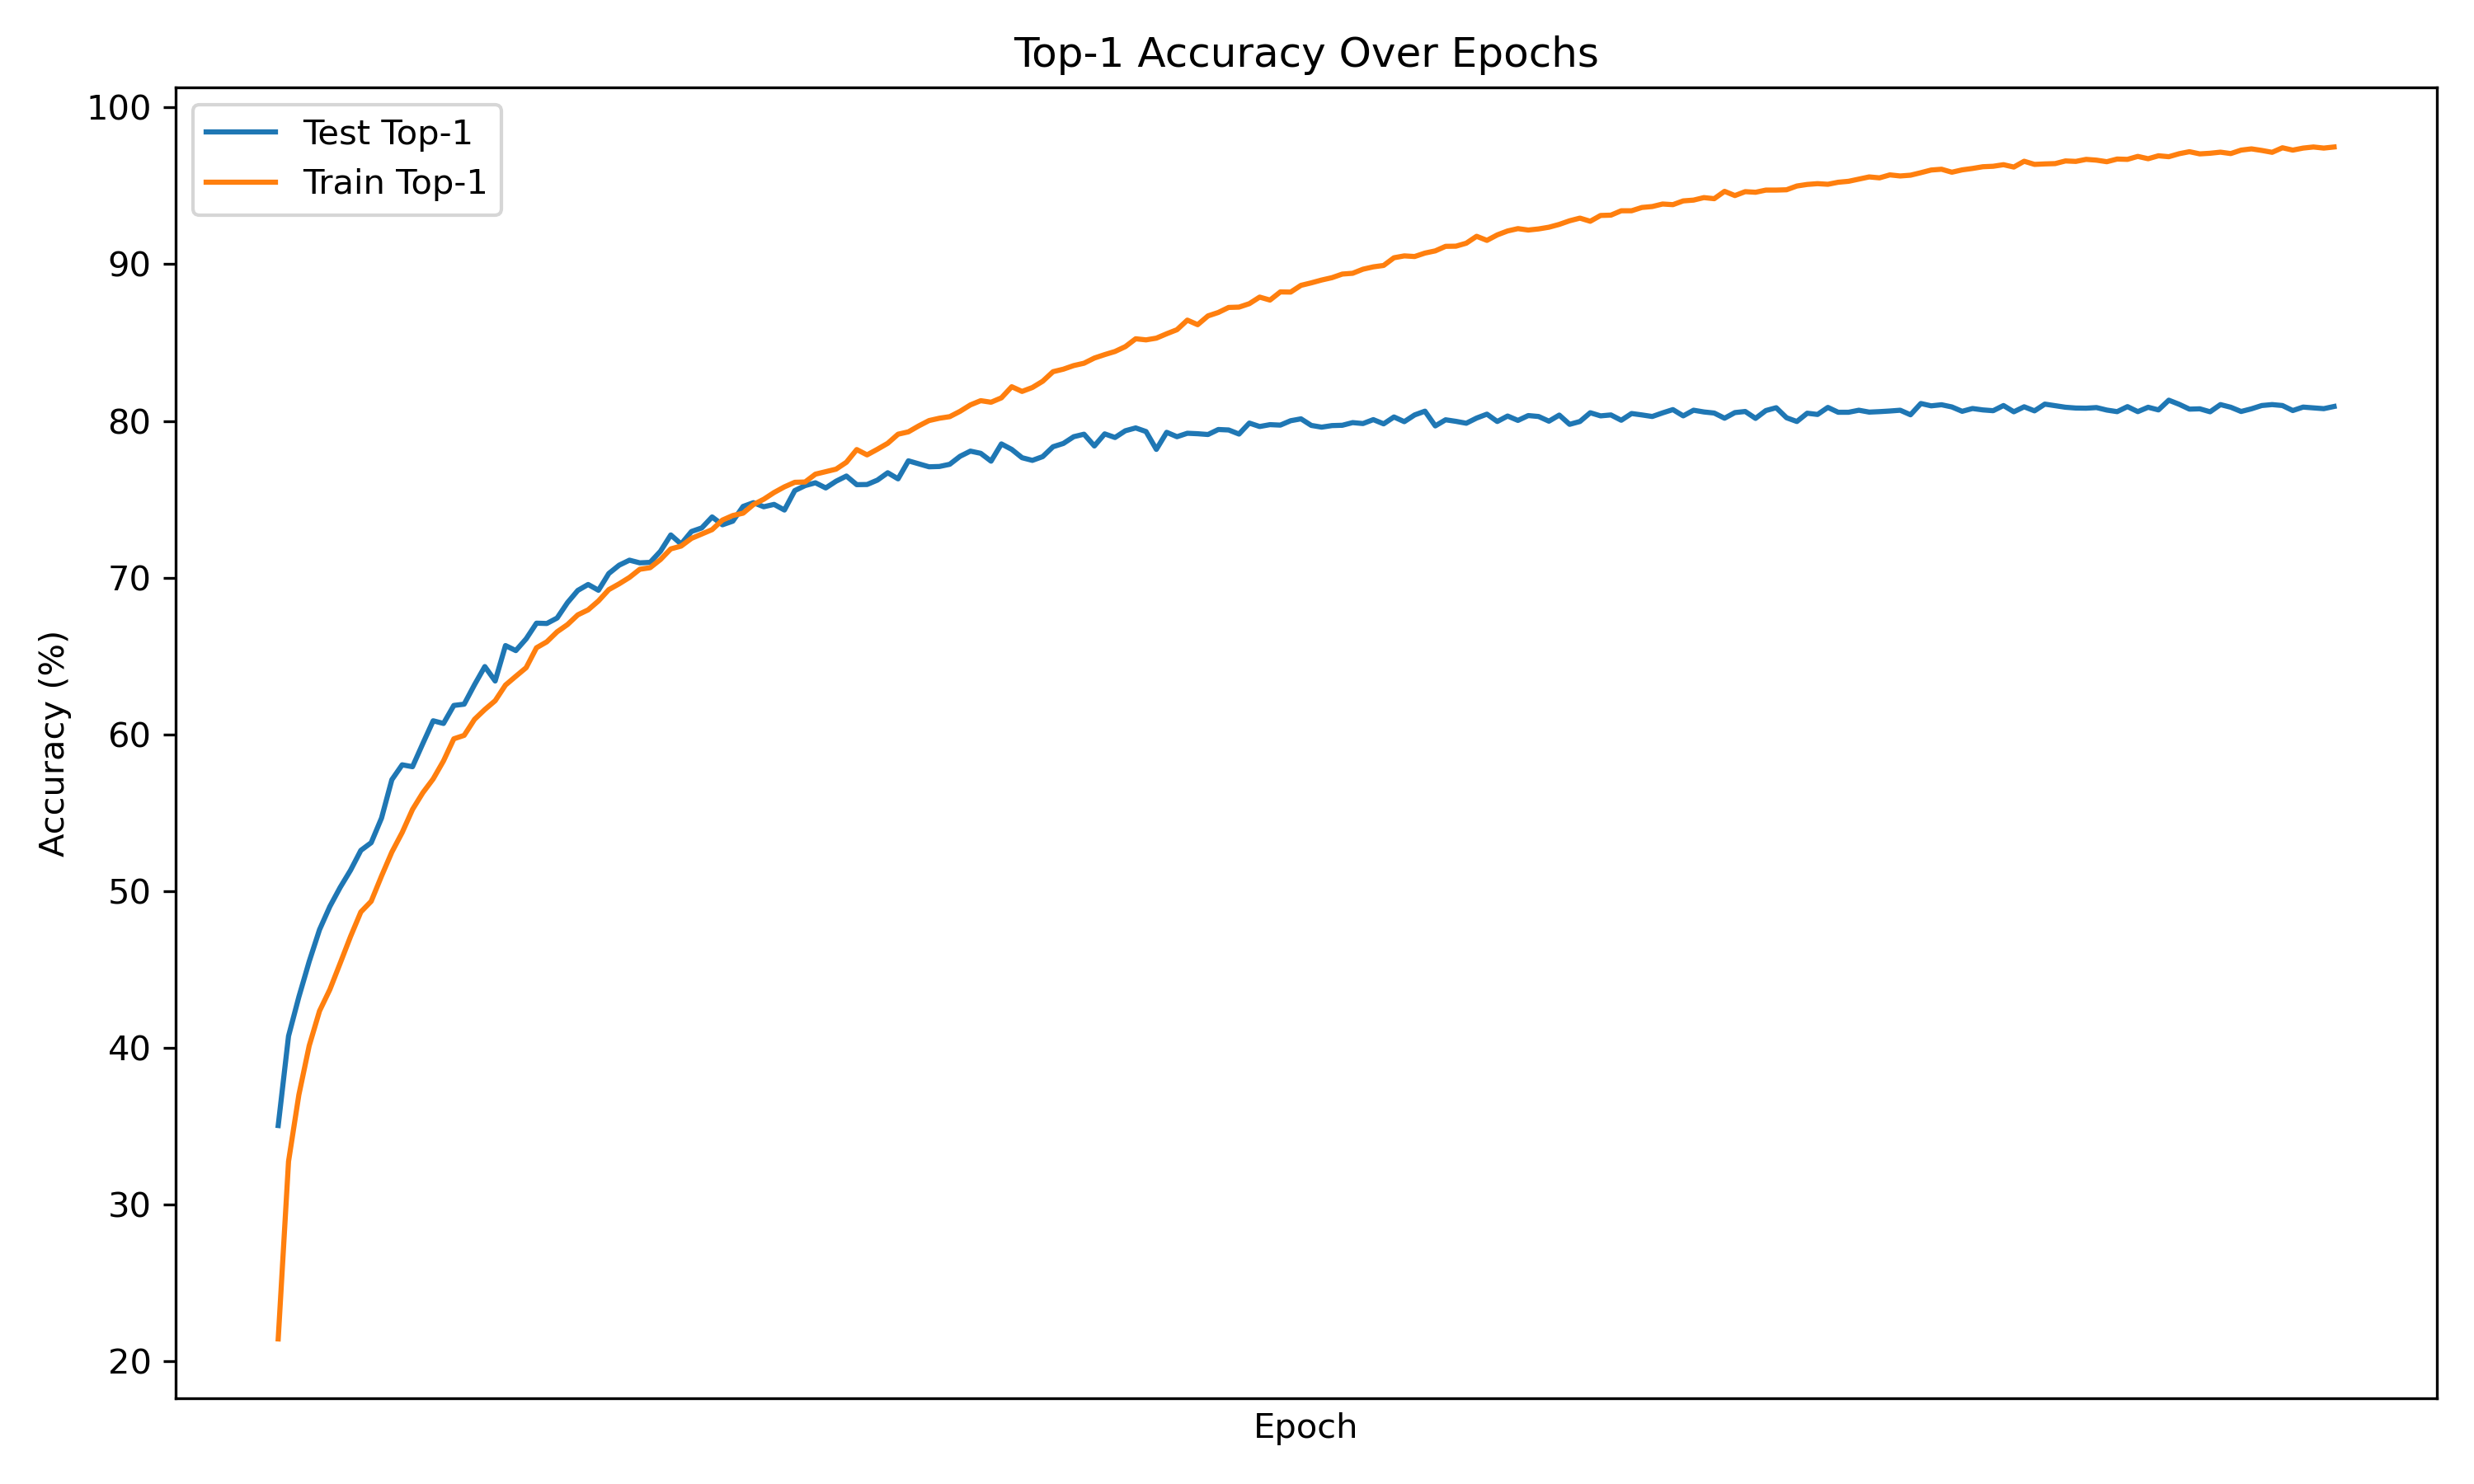
\includegraphics[width=0.85\textwidth]{transformer_images/results/cifar10_swin_original.png}
	\caption{روند تغییرات دقت \lr{Top-1} مدل اصلی \lr{Swin-Tiny} بر روی مجموعه‌داده \lr{CIFAR-10}.}
	\label{fig:cifar10_swin_original}
\end{figure}

\begin{figure}[ht]
	\centering
	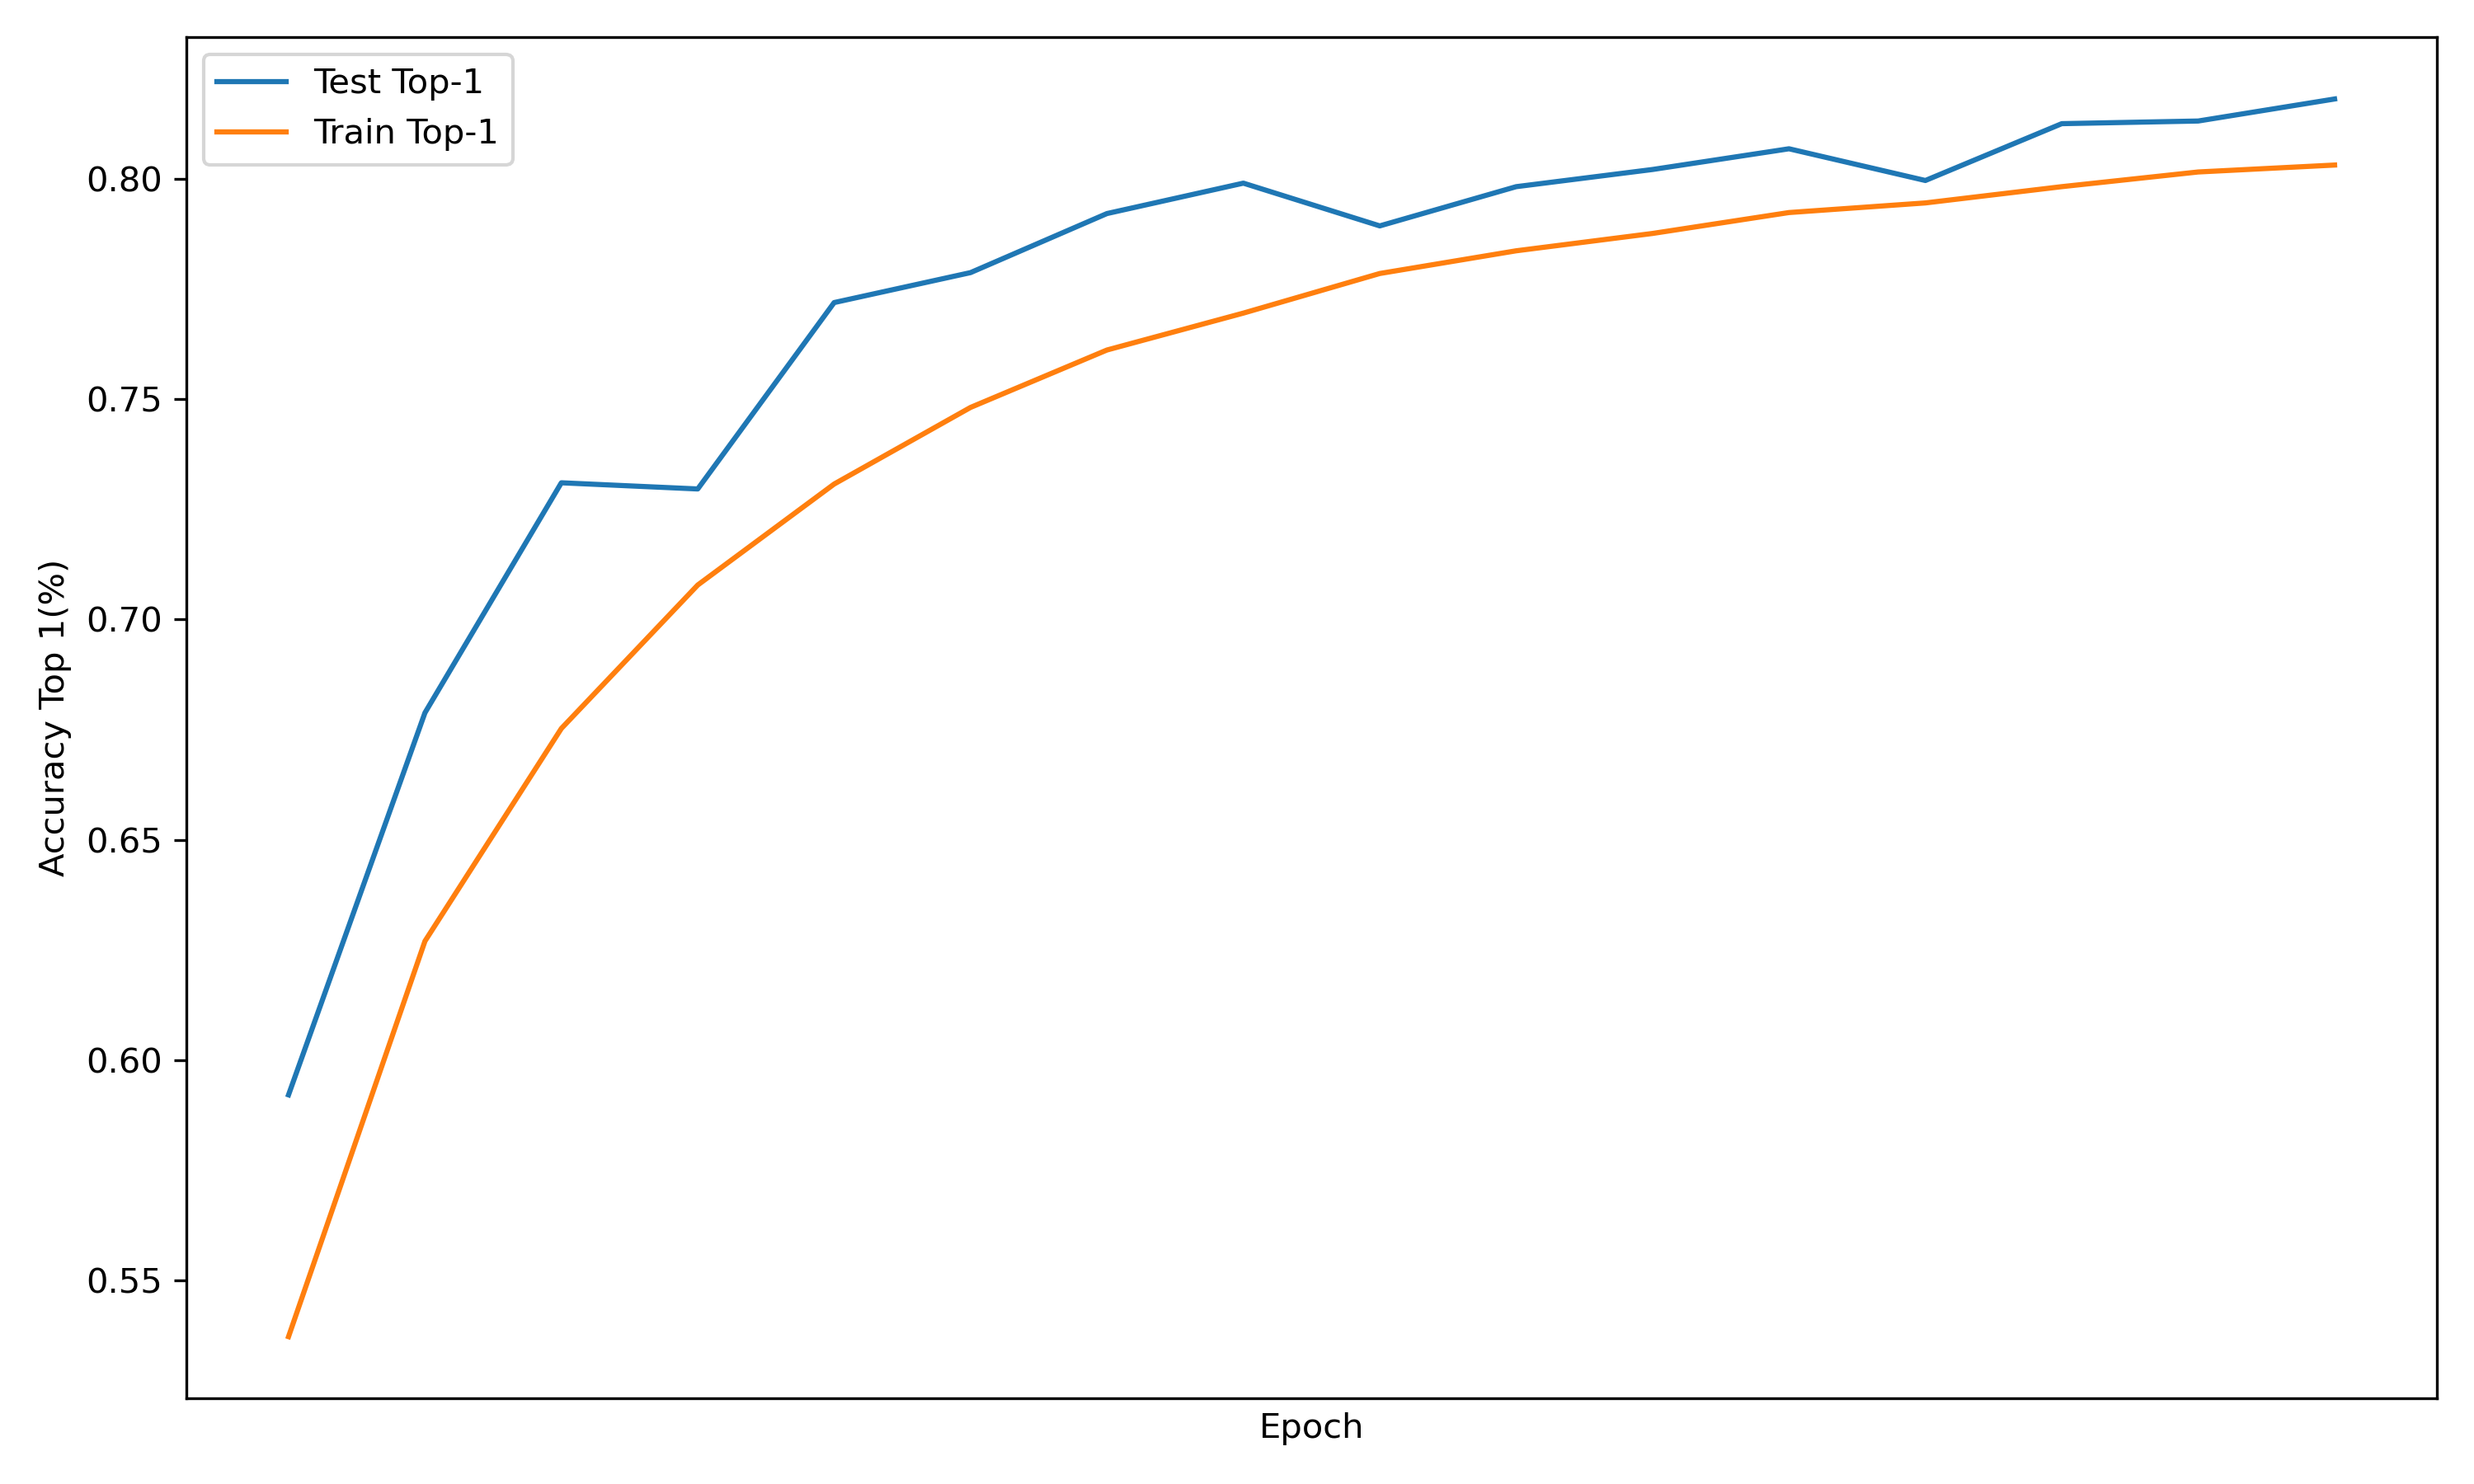
\includegraphics[width=0.85\textwidth]{transformer_images/results/cifar10_tensorized.png}
	\caption{روند تغییرات دقت \lr{Top-1} مدل پیشنهادی \lr{Tensorized Swin} بر روی مجموعه‌داده \lr{CIFAR-10}.}
	\label{fig:cifar10_tensorized}
\end{figure}

\subsection{جمع‌بندی}

در مجموع می‌توان گفت که استفاده از ساختار تانسوری در بخش‌های کلیدی مدل، علاوه بر کاهش چشم‌گیر پیچیدگی محاسباتی و نیاز حافظه، موجب بهبود تعمیم‌پذیری و کاهش بیش‌برازش نیز شده است. این امر اهمیت به‌کارگیری روش‌های فشرده‌سازی ساختاریافته را در طراحی مدل‌های کارا برای کاربردهای کم‌منبع تأیید می‌کند.

% ======================================================
\section{نتایج بر روی دیتاست \lr{MNIST}}

برای ارزیابی عملکرد مدل پیشنهادی بر روی داده‌های ساده‌تر و با ابعاد کوچک‌تر، آزمایش‌ها بر روی دیتاست \lr{MNIST} انجام شده است. در این بخش نیز دو پیکربندی مقایسه شده‌اند: مدل اصلی \lr{Tiny Swin Transformer} و نسخه‌ی پیشنهادی یعنی \lr{Tensorized Swin Transformer}.  

\subsection{خلاصه نتایج کمی}

\begin{table}[ht]
	\centering
	\caption{مقایسه‌ی عملکرد مدل اصلی و مدل تانسوری بر روی \lr{MNIST} (فقط Top-1 و Top-5).}
	\label{tab:mnist_summary_tensor}
	\begin{tabular}{ccccccl}
		\hline
		\multicolumn{2}{c}{تست} & \multicolumn{2}{c}{آموزش} & \multirow{2}{*}{\#پارامترها} & \multirow{2}{*}{مدل} \\
		\cline{1-4}
		Top-5 & Top-1 & Top-5 & Top-1 &  &  \\
		\hline
		\lr{99.9\%} & \lr{97.0\%} & \lr{99.9\%} & \lr{95.8\%} & \lr{27,528,690} & \lr{Tiny Swin} \\
		\lr{100\%} & \lr{98.9\%} & \lr{99.9\%} & \lr{97.3\%} & \lr{1,368,626} & \lr{Tensorized Swin} \\
		\hline
	\end{tabular}
\end{table}

\subsection{نمایش روند آموزش}

شکل‌های \ref{fig:mnist_swin_original} و \ref{fig:mnist_tensorized} روند تغییرات دقت \lr{Top-1} را برای مدل اصلی و مدل تانسوری بر روی مجموعه‌داده‌ی \lr{MNIST} نشان می‌دهند. هر دو مدل به سرعت به دقت بسیار بالا رسیده‌اند، اما مدل تانسوری با وجود تعداد پارامترهای بسیار کمتر، دقت نهایی بالاتری در داده‌های آزمون کسب کرده است.

\begin{figure}[ht]
	\centering
	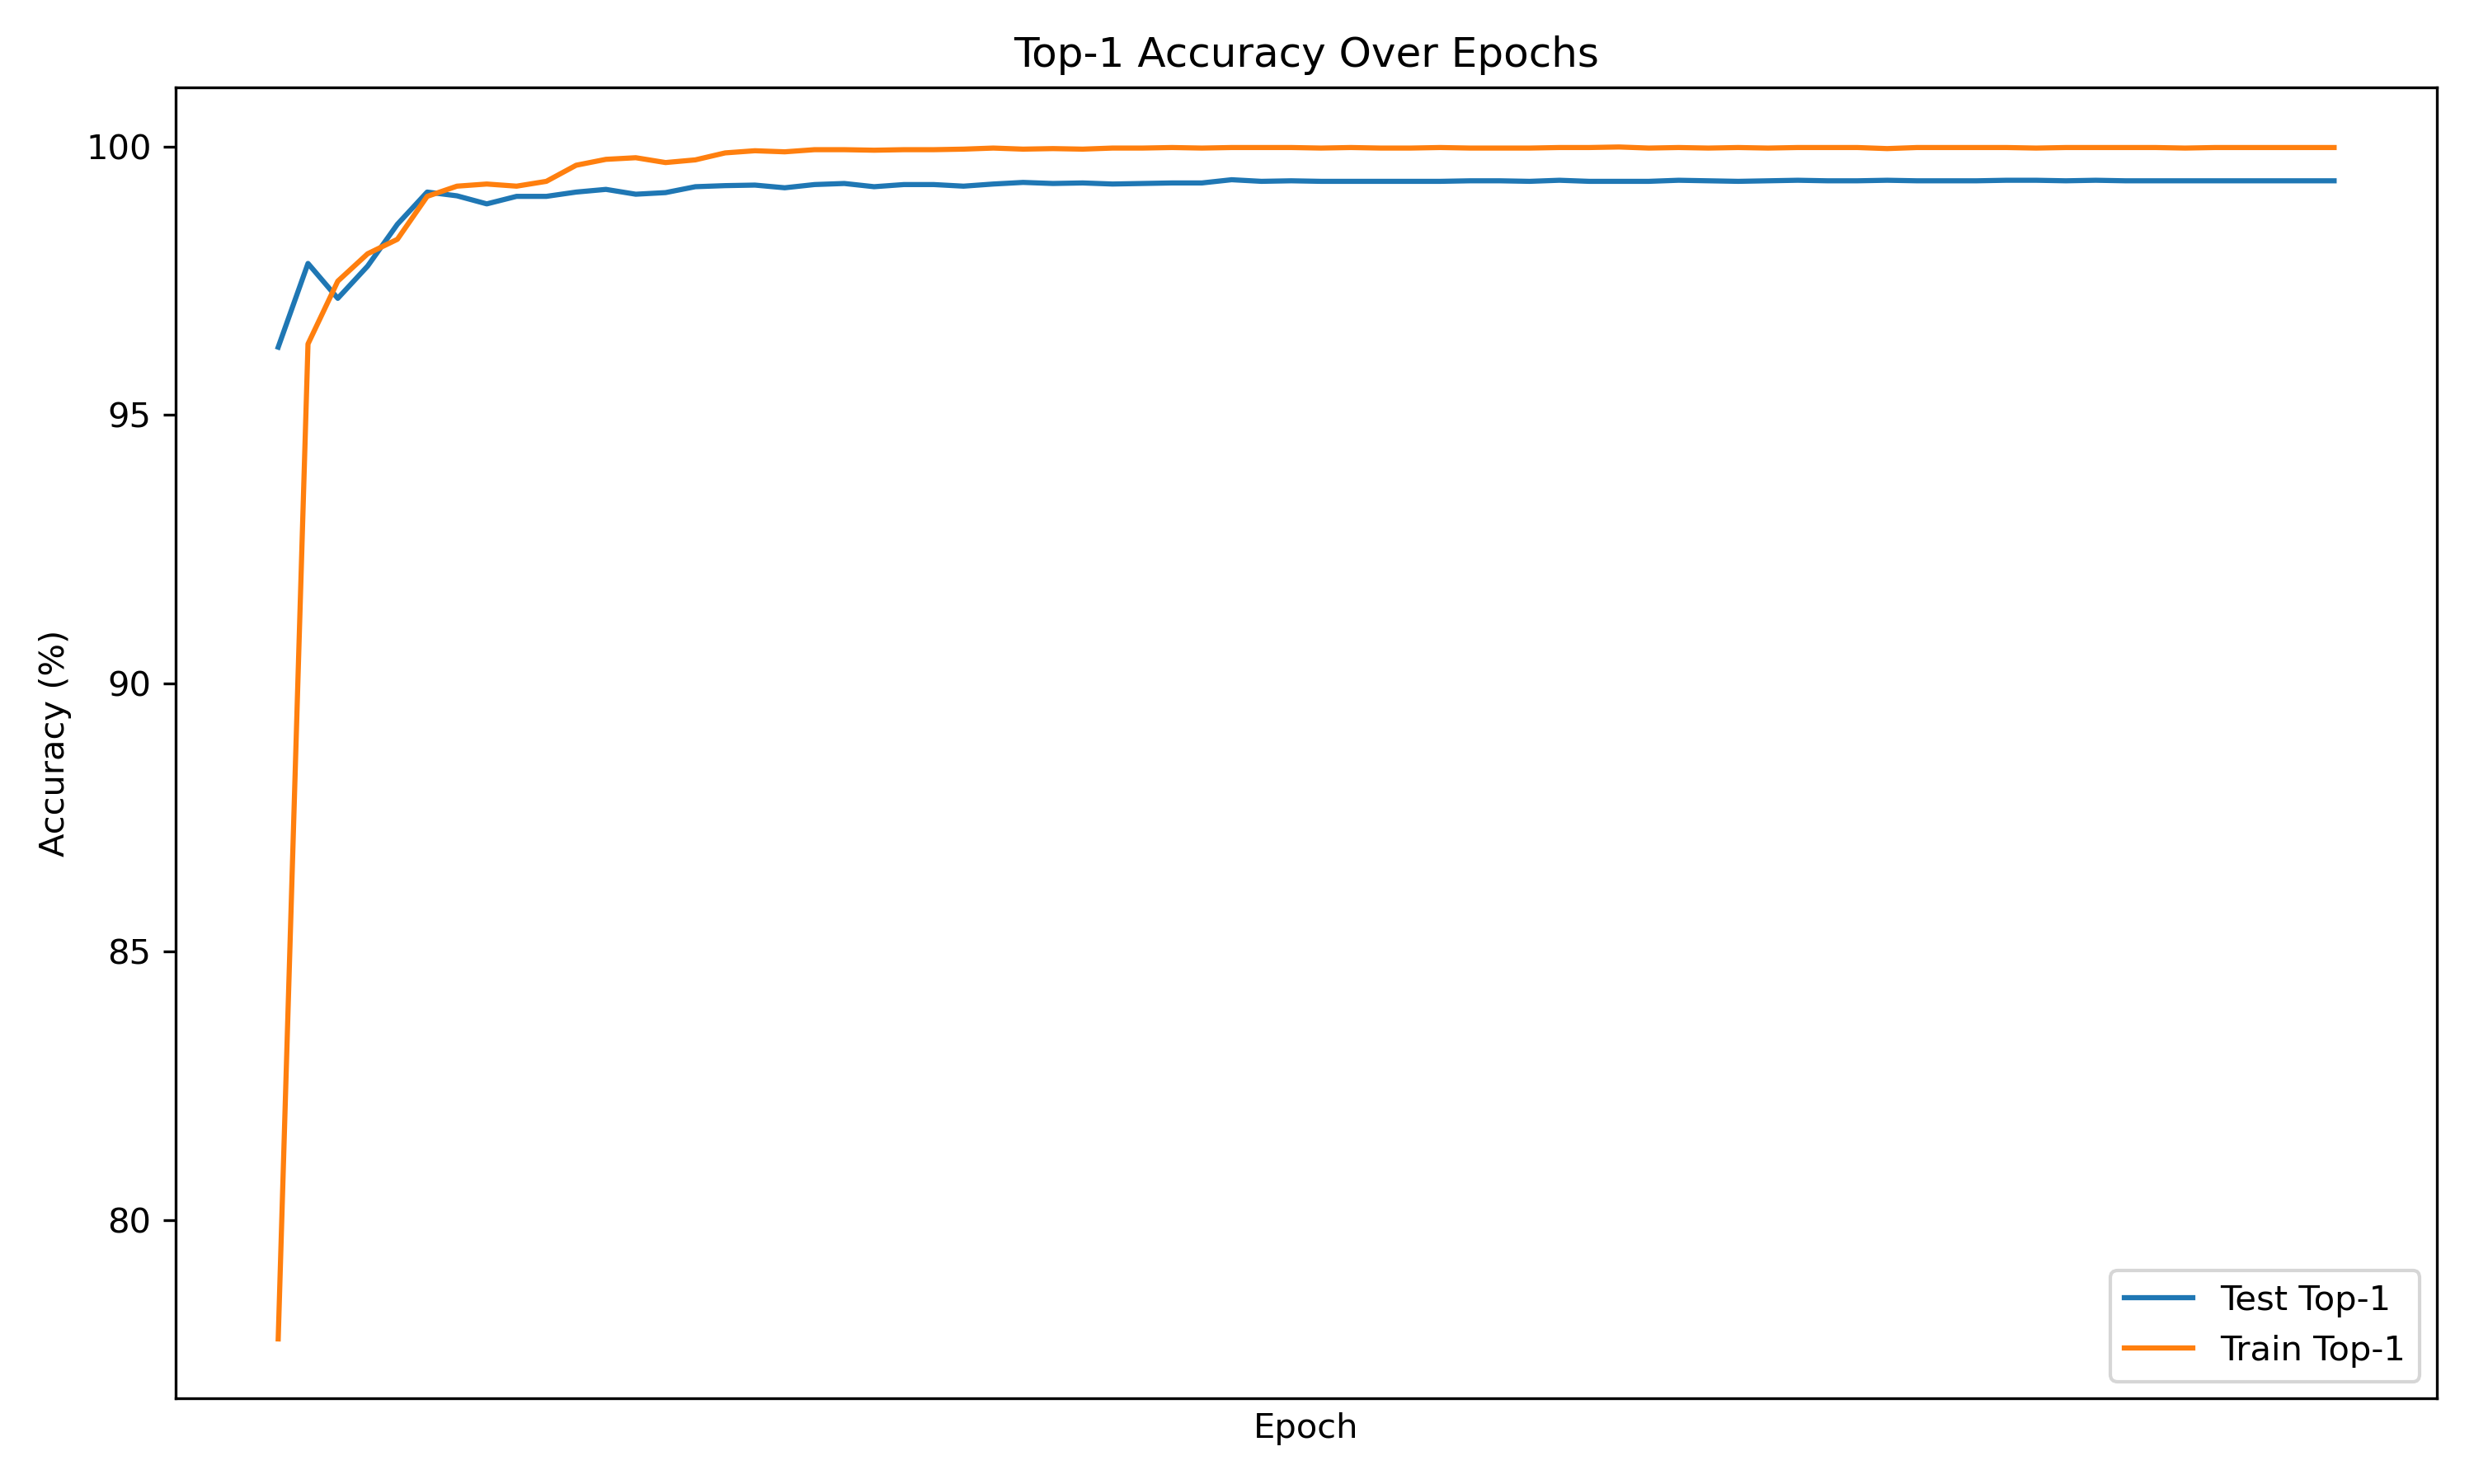
\includegraphics[width=0.85\textwidth]{transformer_images/results/mnist_original.png}
	\caption{روند دقت \lr{Top-1} مدل اصلی \lr{Swin-Tiny} بر روی \lr{MNIST}.}
	\label{fig:mnist_swin_original}
\end{figure}

\begin{figure}[ht]
	\centering
	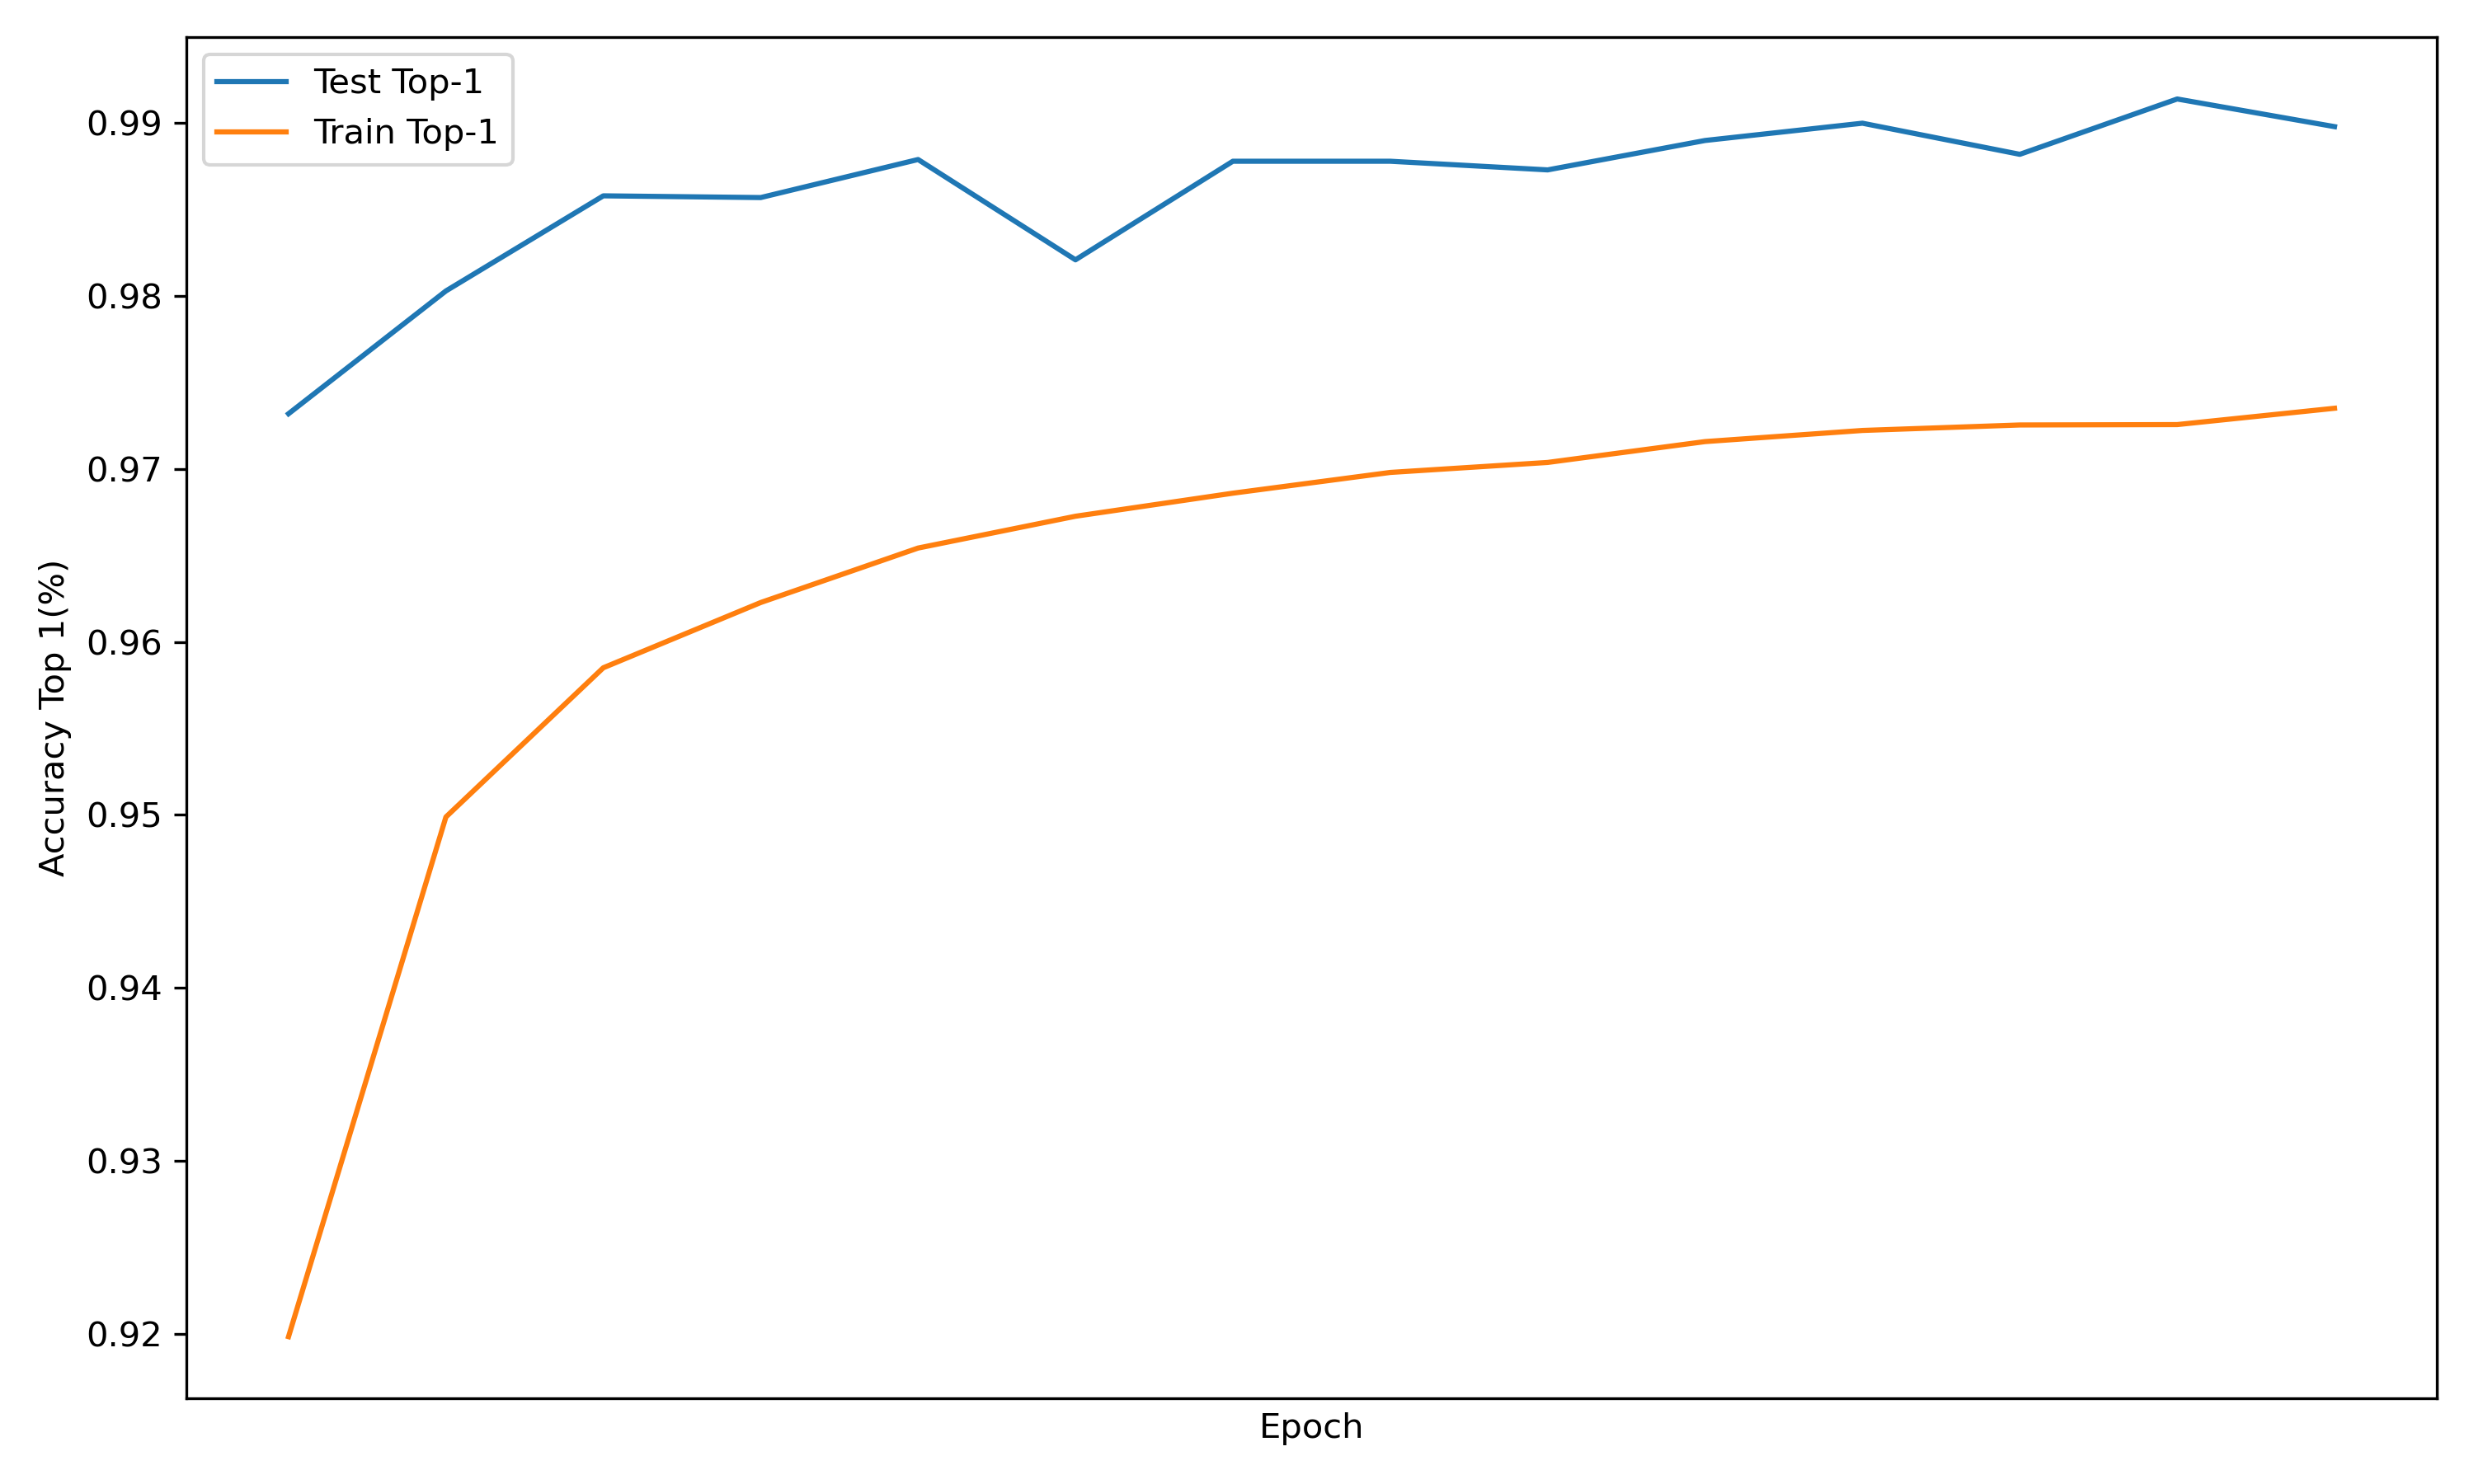
\includegraphics[width=0.85\textwidth]{transformer_images/results/mnist_tensorized.png}
	\caption{روند دقت \lr{Top-1} مدل تانسوری پیشنهادی بر روی \lr{MNIST}.}
	\label{fig:mnist_tensorized}
\end{figure}

\subsection{تحلیل و بحث}

نتایج جدول \ref{tab:mnist_summary_tensor} نشان می‌دهد که مدل تانسوری تنها با \lr{1,368,626} پارامتر توانسته است عملکردی بهتر از مدل اصلی با بیش از \lr{27M} پارامتر ارائه دهد. دقت آزمون در شاخص \lr{Top-1} از \lr{97.0\%} به \lr{98.9\%} افزایش یافته و در شاخص \lr{Top-5} نیز از \lr{99.9\%} به \lr{100\%} رسیده است.  

علاوه بر این، شکاف میان دقت آموزش و آزمون در مدل اصلی حدود \lr{1.2} واحد درصد بوده است، در حالی که در مدل تانسوری این شکاف منفی شده و دقت آزمون بالاتر از دقت آموزش قرار گرفته است. این نشان‌دهنده تعمیم‌پذیری بهتر مدل تانسوری است. حتی در مجموعه‌داده‌ای ساده مانند \lr{MNIST} نیز این بهبود اهمیت دارد، زیرا تأکید می‌کند که فشرده‌سازی تانسوری نه تنها پارامترها را کاهش می‌دهد، بلکه می‌تواند به‌عنوان یک منظم‌ساز مؤثر عمل کند.

\subsection{جمع‌بندی}

به طور کلی، نتایج آزمایش‌ها بر روی دیتاست \lr{MNIST} نشان دادند که مدل تانسوری با کاهش چشمگیر پارامترها نه تنها عملکرد مدل را حفظ کرده بلکه در داده‌های آزمون نیز عملکرد بهتری داشته است. این نتایج اهمیت استفاده از روش‌های تانسوری را حتی در داده‌های ساده تأیید می‌کند.

% ======================================================
\section{نتایج بر روی دیتاست \lr{Tiny ImageNet}}

برای بررسی عملکرد مدل در یک سناریوی چالش‌برانگیزتر، آزمایش‌هایی بر روی دیتاست \lr{Tiny ImageNet} انجام شد. در این بخش علاوه بر مدل اصلی \lr{Tiny Swin Transformer}، مدل پیشنهادی تانسوری نیز با دو بهینه‌ساز متفاوت (\lr{Adam} و \lr{AdamW}) مورد ارزیابی قرار گرفته است.

\subsection{خلاصه نتایج کمی}

\begin{table}[ht]
	\centering
	\caption{مقایسه‌ی عملکرد مدل‌ها بر روی \lr{Tiny ImageNet}.}
	\label{tab:tinyimagenet_summary}
	\begin{tabular}{ccccccc}
		\hline
		\multicolumn{2}{c}{آزمون} & \multicolumn{2}{c}{آموزش} & \#پارامتر & مدل & بهینه‌ساز \\
		\cline{1-4}
		Top-5 & Top-1 & Top-5 & Top-1 &  &  &  \\
		\hline
		\lr{85.42\%} & \lr{64.14\%} & \lr{59.03\%} & \lr{42.26\%} & \lr{27,528,690} & \lr{Tiny Swin} & -- \\
		\lr{54.17\%} & \lr{30.85\%} & \lr{98.50\%} & \lr{83.89\%} & \lr{1,368,626} & \lr{Tensorized Swin} & \lr{Adam} \\
		\lr{62.07\%} & \lr{35.90\%} & \lr{80.90\%} & \lr{55.30\%} & \lr{1,368,626} & \lr{Tensorized Swin} & \lr{AdamW} \\
		\hline
	\end{tabular}
\end{table}

\subsection{نمایش روند آموزش}

شکل \ref{fig:tiny_original_top1} روند تغییر دقت \lr{Top-1} را برای مدل اصلی \lr{Tiny Swin} نشان می‌دهد. همچنین، شکل‌های \ref{fig:tiny_tensor_adam} و \ref{fig:tiny_tensor_adamw} مربوط به مدل تانسوری با بهینه‌سازهای \lr{Adam} و \lr{AdamW} هستند.

\begin{figure}[ht]
	\centering
	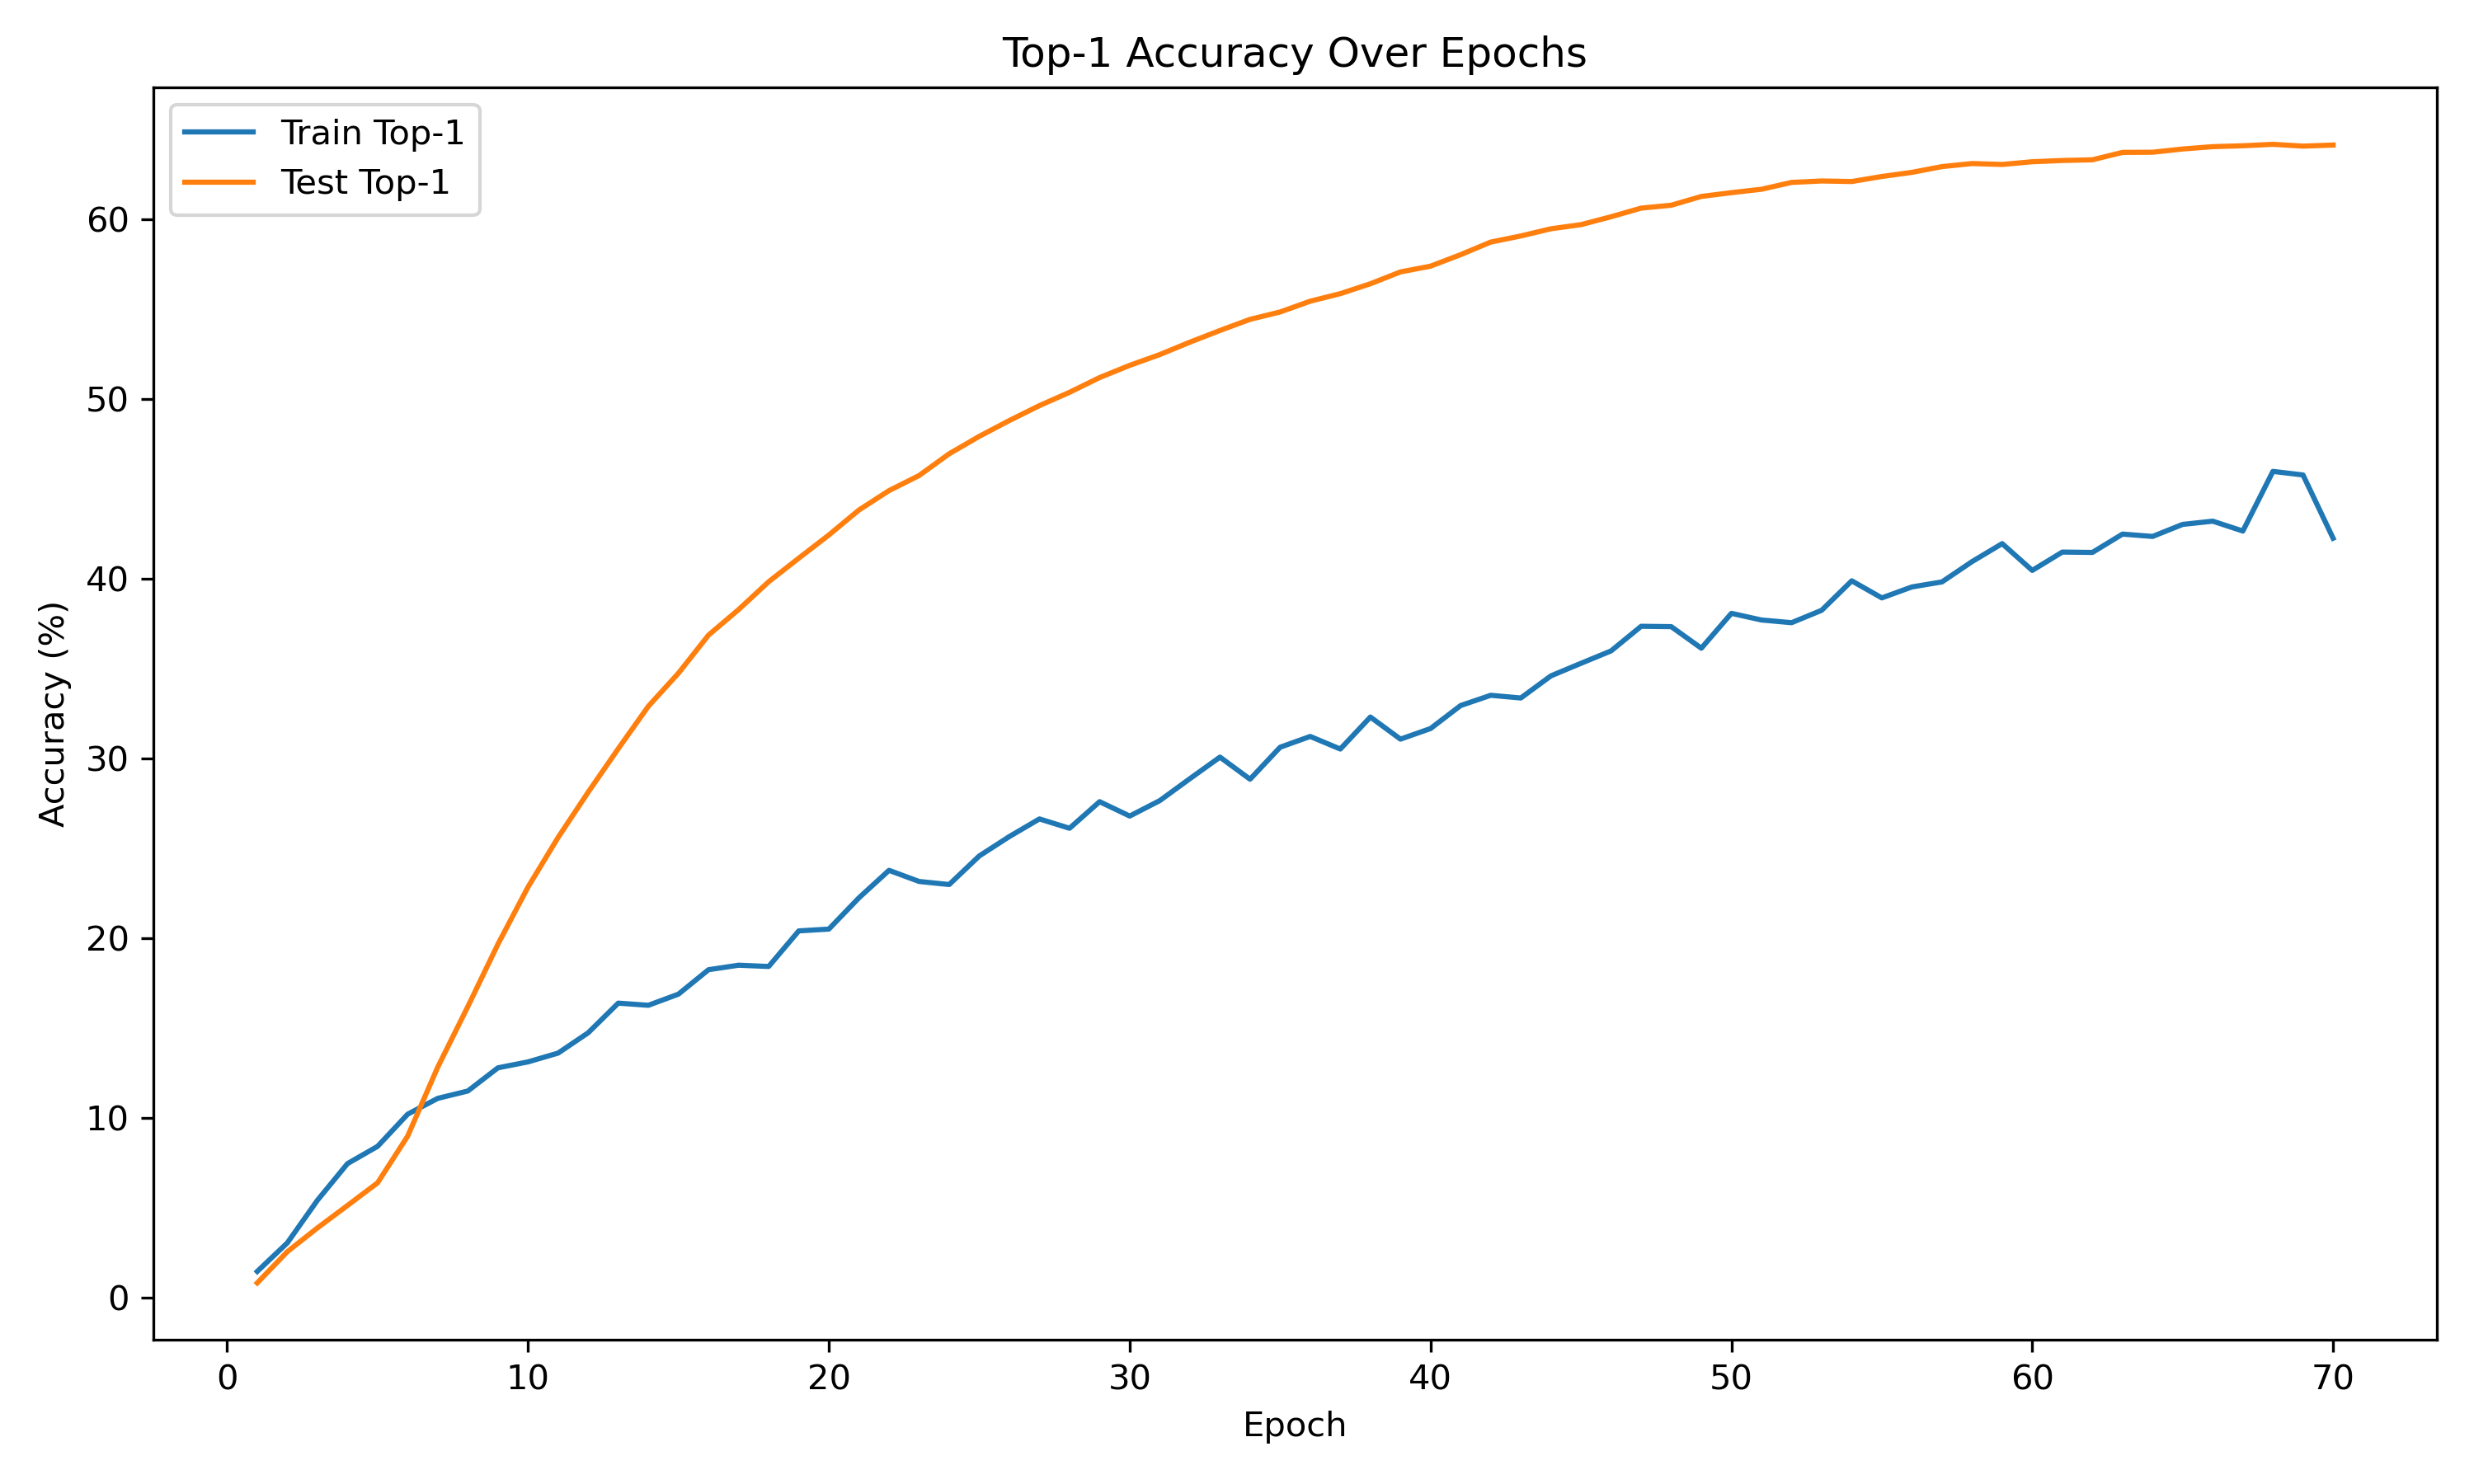
\includegraphics[width=0.85\textwidth]{transformer_images/results/tiny_image_net_original.png}
	\caption{روند دقت \lr{Top-1} مدل اصلی \lr{Swin-Tiny} بر روی \lr{Tiny ImageNet}.}
	\label{fig:tiny_original_top1}
\end{figure}

\begin{figure}[ht]
	\centering
	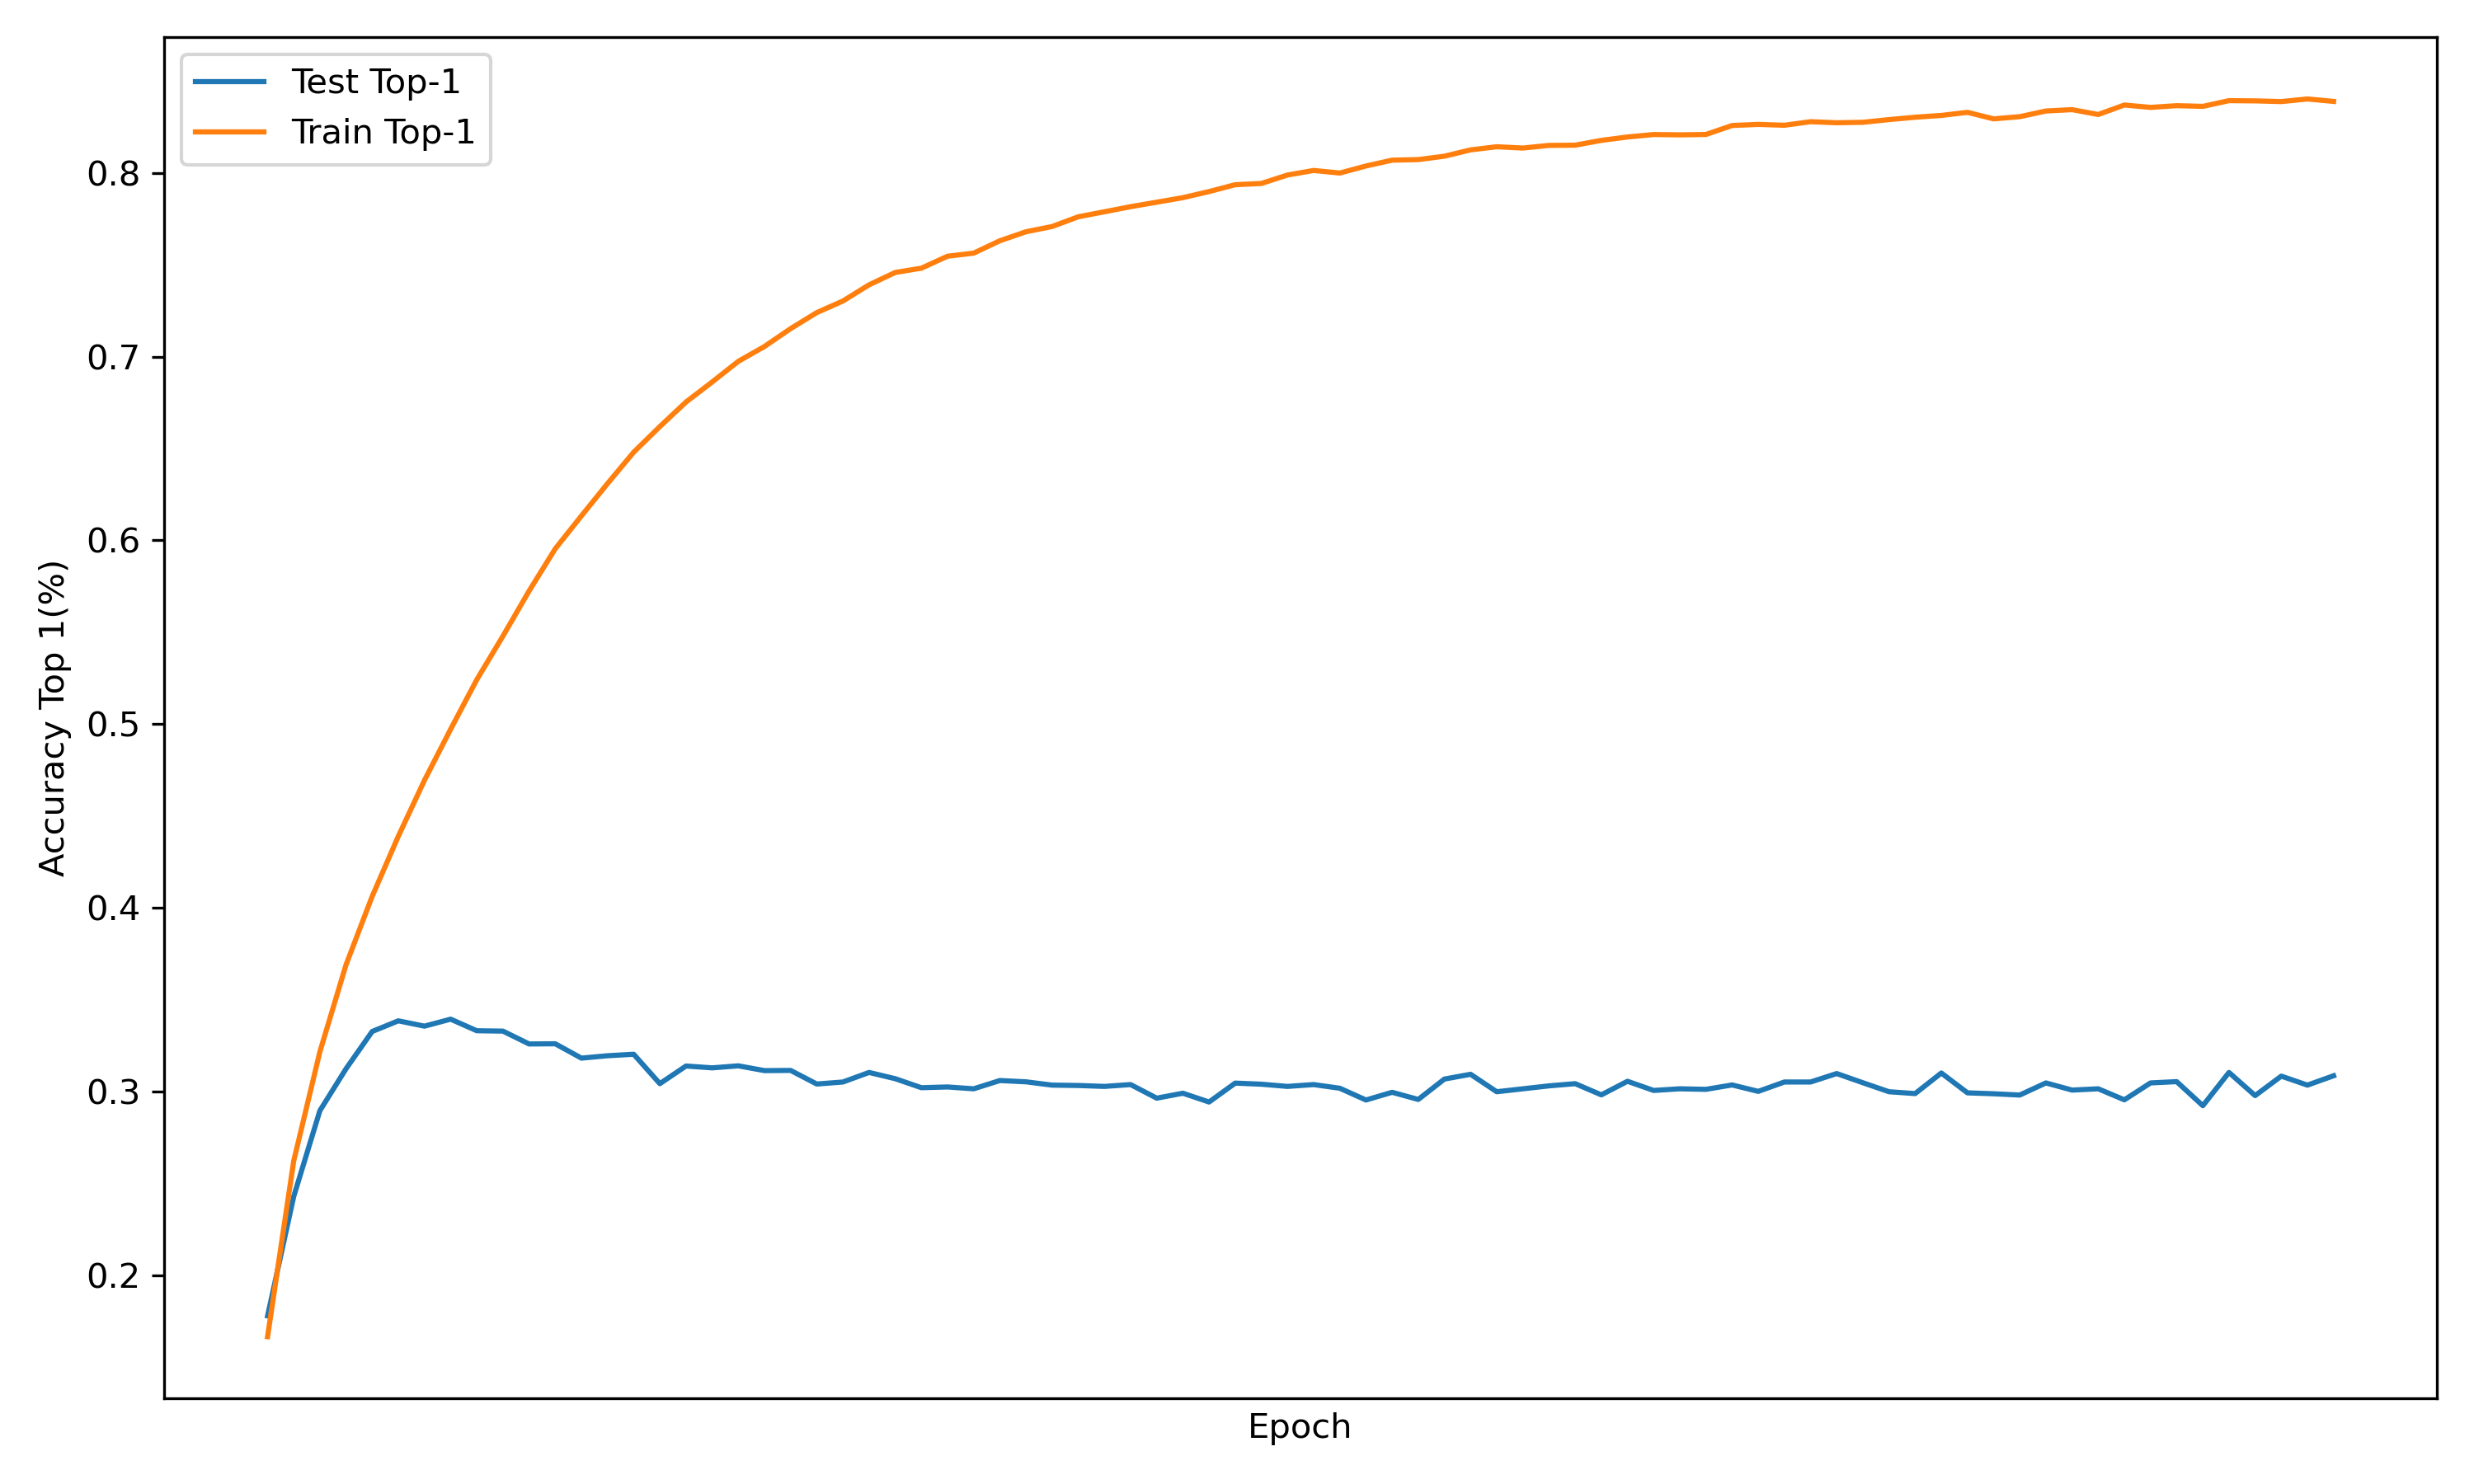
\includegraphics[width=0.85\textwidth]{transformer_images/results/tiny_image_net_tensorized_2.png}
	\caption{روند دقت \lr{Top-1} مدل تانسوری با بهینه‌ساز \lr{Adam} بر روی \lr{Tiny ImageNet}.}
	\label{fig:tiny_tensor_adam}
\end{figure}

\begin{figure}[ht]
	\centering
	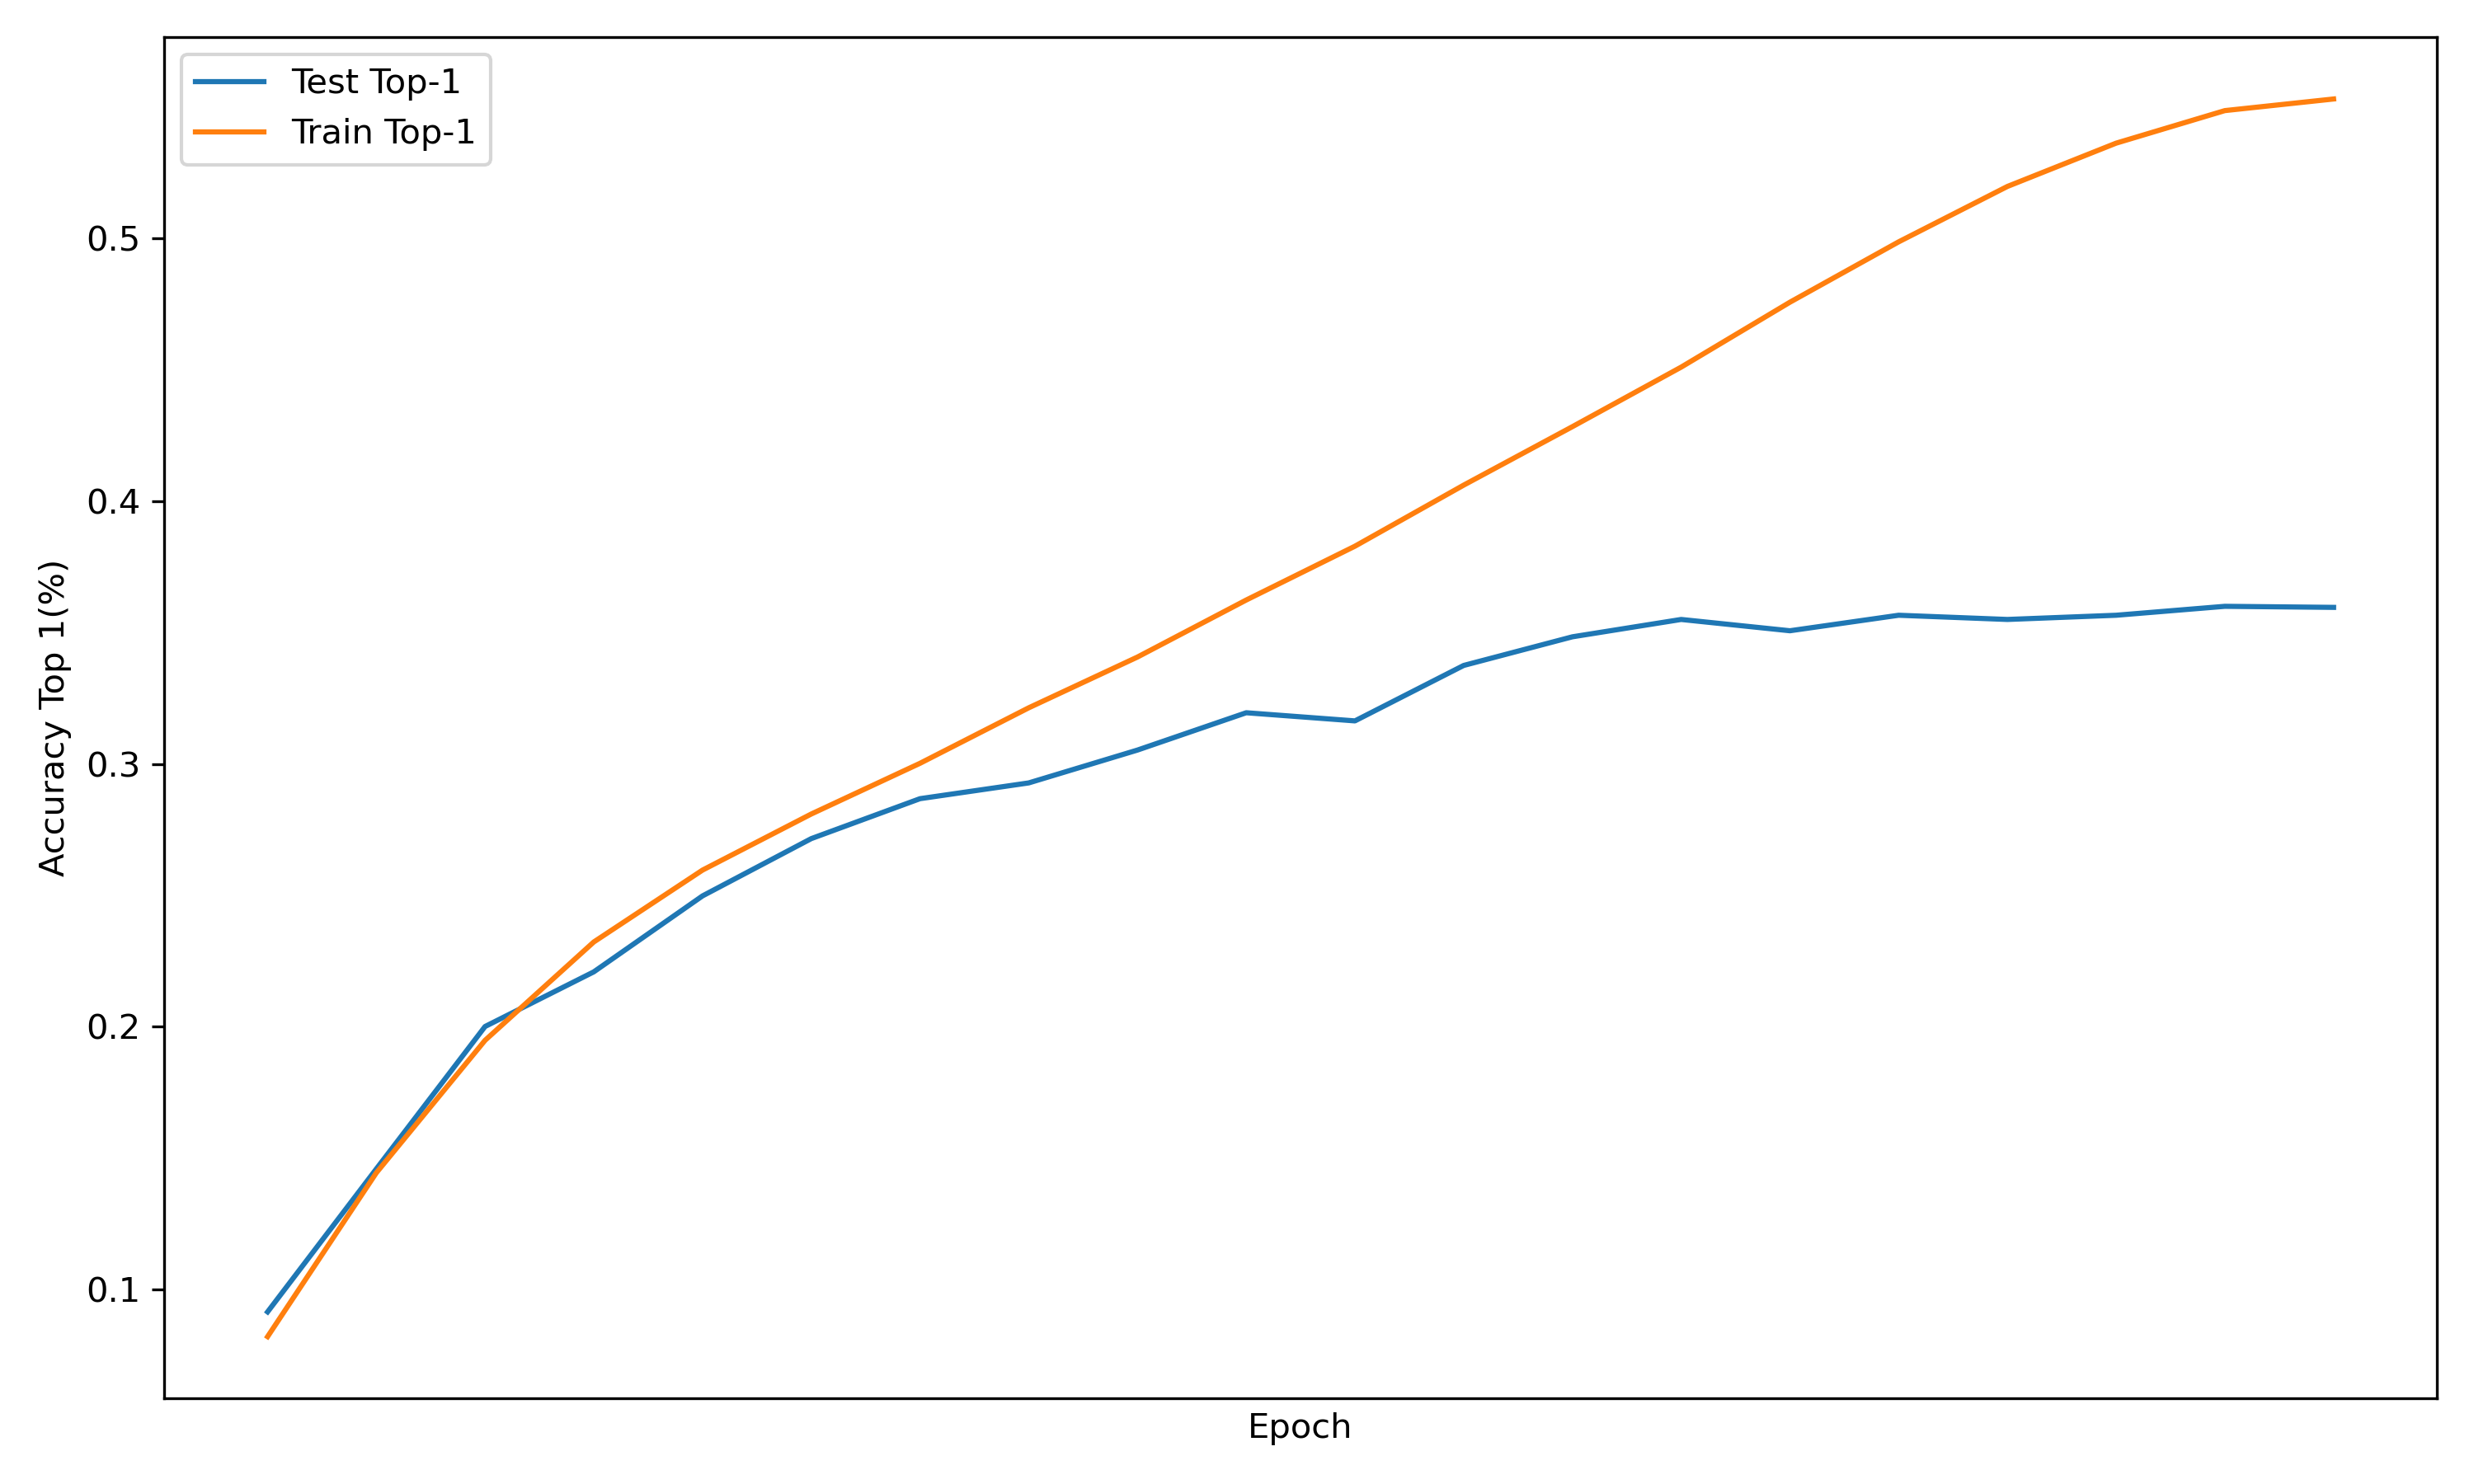
\includegraphics[width=0.85\textwidth]{transformer_images/results/tiny_image_net_tensorized.png}
	\caption{روند دقت \lr{Top-1} مدل تانسوری با بهینه‌ساز \lr{AdamW} بر روی \lr{Tiny ImageNet}.}
	\label{fig:tiny_tensor_adamw}
\end{figure}

\subsection{تحلیل و بحث}

نتایج جدول \ref{tab:tinyimagenet_summary} و نمودارهای مربوطه نشان می‌دهد که رفتار مدل‌ها در این دیتاست پیچیده‌تر متفاوت از دو دیتاست قبلی است. مدل اصلی \lr{Tiny Swin} با داشتن بیش از \lr{27M} پارامتر، دقت آزمون \lr{Top-1} معقولی معادل \lr{64.14\%} به دست آورده است. با این حال اختلاف میان دقت آموزش (\lr{42.26\%}) و آزمون بسیار زیاد است که می‌تواند ناشی از محدودیت در داده‌ها یا تنظیمات بهینه‌سازی باشد.  

مدل تانسوری با بهینه‌ساز \lr{Adam} عملکردی متفاوت نشان داده است. این مدل در داده‌های آموزش به دقت بسیار بالایی (\lr{83.89\%}) رسیده اما در داده‌های آزمون تنها \lr{30.85\%} کسب کرده است، که نشانگر بیش‌برازش شدید است. در مقابل، استفاده از بهینه‌ساز \lr{AdamW} منجر به بهبود نسبی عملکرد شده و دقت آزمون به \lr{35.90\%} افزایش یافته است، هرچند همچنان فاصله‌ی زیادی تا عملکرد مدل اصلی دارد.  

این یافته‌ها بیانگر آن است که کاهش شدید پارامترها در دیتاست‌های پیچیده‌تر مانند \lr{Tiny ImageNet}، در صورت عدم استفاده از منظم‌سازی و استراتژی‌های بهینه‌سازی مناسب، می‌تواند به افت تعمیم‌پذیری منجر شود. 

\subsection{جمع‌بندی}

در مجموع، در حالی که نتایج به‌دست‌آمده روی دو دیتاست \lr{CIFAR-10} و \lr{MNIST} نشان دادند که مدل تانسوری می‌تواند همزمان با کاهش چشمگیر پارامترها عملکرد بهتری نیز ارائه دهد، در دیتاست چالش‌برانگیزتر \lr{Tiny ImageNet} این کاهش ظرفیت موجب افت دقت آزمون شده است. با این حال استفاده از بهینه‌ساز مناسب مانند \lr{AdamW} توانسته است تا حدی شکاف میان آموزش و آزمون را کاهش دهد و مسیری برای تحقیقات آینده در ترکیب روش‌های فشرده‌سازی و بهینه‌سازی پیشنهاد کند.
